% !TeX spellcheck = pt-BR
\documentclass[
	% -- opções da classe memoir --
	12pt,				% tamanho da fonte
%	openright,			% capítulos começam em pág ímpar (insere página vazia caso preciso)
	oneside,			% para impressão em recto e verso. Oposto a oneside
	a4paper,			% tamanho do papel. 
	% -- opções da classe abntex2 --
	%chapter=TITLE,		% títulos de capítulos convertidos em letras maiúsculas
	%section=TITLE,		% títulos de seções convertidos em letras maiúsculas
	%subsection=TITLE,	% títulos de subseções convertidos em letras maiúsculas
	%subsubsection=TITLE,% títulos de subsubseções convertidos em letras maiúsculas
	% -- opções do pacote babel --
	english,			% idioma adicional para hifenização
	french,				% idioma adicional para hifenização
	spanish,			% idioma adicional para hifenização
	brazil,				% o último idioma é o principal do documento
	%article,
	]{abntex2}


% ---
% PACOTES
% ---

% ---
% Pacotes fundamentais 
% ---
\usepackage{lmodern}			% Usa a fonte Latin Modern
\usepackage[T1]{fontenc}		% Selecao de codigos de fonte.
\usepackage[utf8]{inputenc}		% Codificacao do documento (conversão automática dos acentos)
\usepackage{indentfirst}		% Indenta o primeiro parágrafo de cada seção.
\usepackage{color}				% Controle das cores
\usepackage{graphicx}			% Inclusão de gráficos
\usepackage{microtype} 			% para melhorias de justificação
\usepackage{float}
% ---

% ---
% Pacotes adicionais, usados no anexo do modelo de folha de identificação
% ---
\usepackage{multicol}
\usepackage{multirow}
% ---
	
% ---
% Pacotes adicionais, usados apenas no âmbito do Modelo Canônico do abnteX2
% ---
\usepackage{amsmath}
\usepackage{amsthm}
\usepackage{amssymb}
\usepackage{graphicx}
\graphicspath{ {images/} }
\usepackage[colorinlistoftodos]{todonotes}

% not from template
\usepackage{lipsum}
%\usepackage{tikz}
\usepackage{pgfplots}
\usetikzlibrary{shapes,shapes.geometric,arrows,fit,calc,positioning,automata,patterns,matrix,arrows.meta, shapes.geometric, arrows,chains}

\usepackage{verbatim}
\usepackage{blindtext}
\usepackage{enumitem}
\usepackage{multicol}
\usepackage{listings}
\newcommand*{\euler}{\mathrm{e}}

\usepackage{fancyvrb}
\usepackage{hyperref}
\usepackage{relsize}

\usepackage{caption}
\usepackage{subcaption}
\usepackage{multicol}
% ---

% ---
% Pacotes de citações
% ---
\usepackage[brazilian,hyperpageref]{backref}	 % Paginas com as citações na bibl
\usepackage[alf]{abntex2cite}	% Citações padrão ABNT

% --- 
% CONFIGURAÇÕES DE PACOTES
% --- 

% ---
% Configurações do pacote backref
% Usado sem a opção hyperpageref de backref
%\renewcommand{\backrefpagesname}{Citado na(s) página(s):~}
\renewcommand{\backrefpagesname}{}
% Texto padrão antes do número das páginas
\renewcommand{\backref}{}
% Define os textos da citação
\renewcommand*{\backrefalt}[4]{
	\ifcase #1 %
		Nenhuma citação no texto.%
	\or
		Citado na página #2.%
	\else
		Citado #1 vezes nas páginas #2.%
	\fi}%
% ---

%%%% TIKZ HEADERS - Fabio

\tikzset{
	startstop/.style={
		rectangle, 
		rounded corners,
		minimum width=4cm, 
		minimum height=1cm,
		align=center, 
		draw=black, 
		fill=gray!70
	},
	startstop2/.style={
		rectangle, 
		rounded corners,
		minimum width=4cm, 
		minimum height=1cm,
		align=center, 
		draw=black, 
		fill=green!30
	},
	process/.style={
		rectangle, 
		minimum width=4cm, 
		minimum height=1cm, 
		align=center, 
		draw=black, 
		fill=gray!30
	},
	process2/.style={
		rectangle, 
		minimum width=4cm, 
		minimum height=1cm, 
		align=center, 
		draw=black, 
		fill=red!30
	},
	process3/.style={
		rectangle, 
		minimum width=4cm, 
		minimum height=1cm, 
		align=center, 
		draw=black, 
		fill=green!30
	},
	decision/.style={
		rectangle, 
		minimum width=4cm, 
		minimum height=1cm, align=center, 
		draw=black, 
		fill=green!30
	},
	arrow/.style={thick,->,>=stealth},
	dec/.style={
		ellipse, 
		align=center, 
		draw=black, 
		fill=black!30
	},
}

%%% end TIZK HEADERS - Fabio

% ---
% Informações de dados para CAPA e FOLHA DE ROSTO
% ---
\titulo{Atividade Final}
\autor{Bruno Canale \\ Bruno Giordano \\ Fábio T. Sancinetti \\ Wanderson Ferreira}
\local{São Paulo - Brasil}
\data{07 de dezembro de 2016}
\instituicao{%
  Universidade de São Paulo
  \par
  Escola Politécnica
  \par
  Programa de Pós-Graduação em Engenharia Elétrica \par PPGEE }
\tipotrabalho{Atividade Final}
% O preambulo deve conter o tipo do trabalho, o objetivo, 
% o nome da instituição e a área de concentração 
\preambulo{ \textbf{PSI5886} Princípios de Neurocomputação \break \textbf{Professor}: Emílio Del Moral Hernandez \break \break \textbf{Atividade Final}: Redes Neurais Convolucionais }
% ---

% ---
% Configurações de aparência do PDF final

% alterando o aspecto da cor azul
\definecolor{blue}{RGB}{41,5,195}

% informações do PDF
\makeatletter
\hypersetup{
		%pagebackref=true,
		pdftitle={\@title}, 
		pdfauthor={\@author},
		pdfsubject={\imprimirpreambulo},
		pdfcreator={},
		pdfkeywords={PSI5886}{Redes Neurais}{atv\_final}, 
		colorlinks=true,       		% false: boxed links; true: colored links
		linkcolor=black,          	% color of internal links
		citecolor=black,        	% color of links to bibliography
		filecolor=black,      		% color of file links
		urlcolor=black,
		bookmarksdepth=4
}
\makeatother
% --- 

% --- 
% Espaçamentos entre linhas e parágrafos 
% --- 

% O tamanho do parágrafo é dado por:
\setlength{\parindent}{1.3cm}

% Controle do espaçamento entre um parágrafo e outro:
\setlength{\parskip}{0.2cm}  % tente também \onelineskip

% ---
% compila o indice
% ---
\makeindex
% ---


% --- styles

\tikzstyle{input}=[draw,fill=white!50,circle,minimum size=20pt,inner sep=0pt]
\tikzstyle{hidden}=[draw,fill=white!50,circle,minimum size=20pt,inner sep=0pt]
\tikzstyle{output}=[draw,fill=white!50,circle,minimum size=20pt,inner sep=0pt]
\tikzstyle{bias}=[draw,dashed,fill=gray!50,circle,minimum size=20pt,inner sep=0pt]

\tikzstyle{stateTransition}=[->, thick]


\usepackage{afterpage}

% ----
% Início do documento
% ----
\begin{document}

% Seleciona o idioma do documento (conforme pacotes do babel)
%\selectlanguage{english}
\selectlanguage{brazil}

% Retira espaço extra obsoleto entre as frases.
\frenchspacing 

% ----------------------------------------------------------
% ELEMENTOS PRÉ-TEXTUAIS
% ----------------------------------------------------------
% \pretextual

% ---
% Capa
% ---
%\imprimircapa
% ---

% ---
% Folha de rosto
% (o * indica que haverá a ficha bibliográfica)
% ---
\imprimirfolhaderosto
% ---

% ---
% inserir lista de tabelas
% ---
%\pdfbookmark[0]{\listtablename}{lot}
%\listoftables*
%\cleardoublepage
% ---

% ---
% inserir lista de abreviaturas e siglas
% ---
\begin{siglas}
	\item[CNN] \textit{Convolutional Neural Networks} - Redes Neurais Convolucionais
	\item[GPU] \textit{Graphic Processor Unit} - Unidade de Processamento Gráfico
	\item[MLP] \textit{Multilayer Perceptron} - Perceptron em muti-camadas
	\item[RNA] Redes Neurais Artificiais
	\item[RNN] \textit{Recurrent Neural Networks} - Redes Neurais Recorrentes
\end{siglas}
% ---

% ---
% inserir lista de símbolos
% ---
%\begin{simbolos}
%  \item[$ \Gamma $] Letra grega Gama
%  \item[$ \Lambda $] Lambda
%  \item[$ \zeta $] Letra grega minúscula zeta
%  \item[$ \in $] Pertence
%\end{simbolos}
% ---

% ---
% inserir o sumario
% ---
\pdfbookmark[0]{\contentsname}{toc}
\tableofcontents*
%\cleardoublepage

% ---


% ----------------------------------------------------------
% ELEMENTOS TEXTUAIS
% ----------------------------------------------------------
\textual

% ----------------------------------------------------------
% Introdução (exemplo de capítulo sem numeração, mas presente no Sumário)
% ----------------------------------------------------------
\chapter[Introdução]{Introdução}

\par A motivação para realizar esse trabalho partiu dos estudos de Redes Neurais Artificiais durante a disciplina. O relacionamento entre Redes Neurais clássicas como as \textit{Multilayer Perceptrons} e \textit{Redes de Hopfields} com redes mais sofisticadas utilizadas na área de \textbf{Deep Learning} não é muito simples de entender a primeira vista. Dessa forma, a proposta desse trabalho foi definida como uma análise aprofundada de algoritmos de Deep Learning.

\par Porém para atingir esse objetivo foi necessário escolher apenas uma arquitetura da classe de algoritmos apresentados na literatura da área. As Redes Neurais Convolucionais apareceram naturalmente como uma ferramenta para visualizar como a informação se transforma ao caminhar para porções cada vez mais profundas do algoritmo de Rede Neural.

\par A ideia do trabalho gira em torno do entendimento do processo de funcionamento de redes convolucionais, porém é suficiente para gerar uma boa intuição de como redes neurais genéricas funcionam e como a abstração da informação pode ser representada de uma camada para a outra. Dessa forma, o estudo permite que o conhecimento adquirido durante a confecção e leitura do trabalho sejam extrapolados para outras arquiteturas de redes neurais.
	

\chapter{Multi-Layer Perceptrons}


\section{Perceptron de Rosenblatt}
O perceptron de Rosenblatt foi uma das primeiras unidades de processamento baseada em neurônios biológicos, implementando classificadores mimetizando o funcionamento do cérebro de seres vivos. Esse perceptron foi a base do desenvolvimento de toda teoria de redes neurais. Analisemos nessa seção esse perceptron, sob um ponto de vista matemático. Considere uma variável de saída $y \in \mathbb{R}$ para entradas $\vec{x} \in \mathbb{R}^m$:

\begin{center}
	\includegraphics[scale=1]{rosenblattperceptron.png}
	\captionof{figure}{ Perceptron de Rosenblatt \cite{livronnet} }
\end{center} 

Matematicamente, temos:

$$ y = \varphi\bigg(  \big(\sum_{i=0}^m w_ix_i\big) + b \bigg)$$

A função de ativação $\varphi$ utilizada por Rosenblatt em sua formulação clássica é a $sgn$, devolvendo resultados entre $+1$ e $-1$ conforme o sinal da entrada:

$$sgn(z) = \begin{cases}
+1 \enspace \text{se } z > 0 \\
-1 \enspace \text{se } z < 0 \\
\end{cases}$$

Reorganizando a equa\c{c}\~ao matricialmente:
$$ \vec{x} = \begin{bmatrix}
x_1 \\
x_2 \\
... \\
x_m
\end{bmatrix},
\vec{w} = \begin{bmatrix}
w_1 \\
w_2 \\
... \\
w_m
\end{bmatrix} \Rightarrow
y = sgn\bigg( \big(\vec{w}^T\cdot \vec{x}\big) + b \bigg)$$

Assim, o output $y$ pode ser associado à duas classes $\mathcal{C}_1$ e $\mathcal{C}_2$, para os respectivos valores $+1$ e $-1$. Como a opera\c{c}\~ao envolvendo os inputs \'e puramente linear, h\'a uma correspond\^encia geom\'etrica interessante facilmente visualiz\'avel para duas dimens\~oes. Considerando um conjunto de dados com duas dimens\~oes, cada input $(x_1,x_2)$ pode ser plotado no $\mathbb{R}^2$. Assim, interpretando os par\^ametros $(\vec{w},b)$ do sistema como vetores:

\begin{center}
	\includegraphics[scale=1]{perceptron2d.png}
	\captionof{figure}{ Interpreta\c{c}\~ao geom\'etrica para duas dimens\~oes \cite{livronnet} }
\end{center} 

Os pesos $(\vec{w},b)$ separam o espa\c{c}o de inputs em duas regi\~oes correspondentes a cada classe $\mathcal{C}_1$ e $\mathcal{C}_2$. Dado um conjunto $D$ de $N$ dados:
$$D = \begin{bmatrix}
d_1 \\
d_2 \\
... \\
d_N
\end{bmatrix} =
\begin{bmatrix}
(X_{ref},Y_{ref})_1 \\
(X_{ref},Y_{ref})_2 \\
... \\
(X_{ref},Y_{ref})_N
\end{bmatrix}$$
Para $d_i = (X_{ref},Y_{ref})_i$ com inputs $X \in \mathbb{R}^m$ e outputs $Y \in \{\{+1\},\{-1\}\}$, queremos então determinar $W$ separando o $\mathbb{R}^m$ em duas regiões $\mathcal{R}_1$ e $\mathcal{R}_2$, cada uma responsável por cada classe definida em $Y$. Ou seja:
$$\forall d_i = (X_{ref},Y_{ref})_i \text{,}  \enspace \enspace \begin{cases}
Y_{ref} = +1 \Leftarrow \Rightarrow X_{ref} \in R_1 \\
Y_{ref} = -1 \Leftarrow \Rightarrow X_{ref} \in R_2 \\
\end{cases} $$


Para estender a formula\c{c}\~ao para um n\'umero arbitr\'ario de classes, podemos utilizar mais neur\^onios. Assim, podemos definir um n\'umero qualquer de regi\~oes utilizando composi\c{c}\~oes de l\'ogica booleana. A combinação de diversos perceptrons e a generalização da função de transferência do neurônio resultou no desenvolvimento da teoria de Multi-Layer Perceptrons.

\section{Multi-Layer Perceptrons}
O Perceptron da arquitetura MLP \'e uma generalização do perceptron de Rosenblatt, utilizando diversos perceptrons de Rosenblatt com fun\c{c}\~oes de ativa\c{c}\~ao $\varphi(.)$ mais gen\'ericas, organizados em diversas camadas. Alguns exemplos de fun\c{c}\~oes $\varphi(.)$ cont\'inuas e diferenci\'aveis utilizadas:

$$\varphi(x) = \begin{cases}
tgh(x) = \frac{ e^x - e^{-x} } {e^x + e^{-x}} \\
sig(x) = \frac{ 1 } {1 + e^{-x}} \\

\end{cases} $$

Tais caracter\'isticas s\~ao as principais respons\'aveis pelos excelentes resultados recentes em aplica\c{c}\~oes de MLP, como tamb\'em s\~ao os principais motivos pela dificuldade no entendimento do comportamento desse tipo de rede neural. A presen\c{c}a de tantas n\~ao linearidades distribuidas combinadas com a alta conectividade entre neur\^onios faz com que a an\'alise te\'orica seja extremamente complexa. Al\'em disso, o uso de camadas escondidas torna o processo de aprendizado extremamente dificil de se visualizar.

Considere o diagrama a seguir de uma MLP com inputs $\vec{x} \in \mathbb{R}^m$ e outputs $\vec{y} \in \mathbb{R}^3$. Sejam duas camadas escondidas: $W_1$ com $n_1$ outputs $h_1 \in \mathbb{R}^{n_1}$ e $W_2$ com $n_2$ outputs $h_2 \in \mathbb{R}^{n_2}$.

\begin{center}
	\includegraphics[scale=0.8]{MLP.png}
	\captionof{figure}{ Diagrama de arquitetura de uma MLP \cite{livronnet} }
\end{center} 

Seja $w_{nij}$ o peso conectando o i-\'esimo neur\^onio da n-\'esima camada ao j-\'esimo output da camada anterior. Analisemos o output $h_{1i}$ do i-\'esimo neur\^onio da primeira camada escondida.  Similarmente ao perceptron de Rosenblatt, considerando uma fun\c{c}\~ao de ativa\c{c}\~ao $\varphi(.)$, temos:

$$h_{1i} =  \varphi \bigg( \sum_{j=0}^m w_{1ij} x_j  \bigg) = \varphi \big(\vec{w_{1i}}^T \cdot \vec{x} ) $$

Onde $\vec{x} = \begin{bmatrix}
x_1 & x_2 & ... & x_m
\end{bmatrix}^T$ denotam os inputs e $\vec{w_{1i}} = \begin{bmatrix}
w_{1i1} & w_{1i2} & ... & w_{1im} \end{bmatrix}^T$ denotam os pesos ligando os inputs ao i-\'esimo neur\^onio da primeira camada. Seja $\vec{h_1} = \begin{bmatrix}
h_{11} &
h_{12} &
... &
h_{1 n_1}
\end{bmatrix}^T$ o vetor contendo todos os outputs dos neur\^onios da primeira camada. Analogamente, analisemos simplificadamente o output $h_{2i}$ do i-\'esimo neur\^onio da segunda camada escondida:

$$h_{2i} = \varphi \big( \vec{w_{2i}}^T \cdot \vec{h_1}  ) = 
\varphi \bigg(
\begin{bmatrix}
w_{2i1} & w_{2i2} & ... & w_{2in_1}
\end{bmatrix} \cdot 
\begin{bmatrix}
\varphi \big(\vec{w_{11}}^T \cdot \vec{x} ) \\
\varphi \big(\vec{w_{12}}^T \cdot \vec{x} ) \\

...  \\
\varphi \big(\vec{w_{1n_1}}^T \cdot \vec{x} )
\end{bmatrix} 
\bigg) \Rightarrow
$$
$$ h_{2i} = \varphi \bigg(
\sum_{j = 0}^{n_1} \big(w_{2ij}\big) \varphi \big(\vec{w_{1j}}^T \cdot \vec{x} )  
\bigg) $$

Finalmente, analisando o output $y_i$ de maneira similar:

$$y_i = \varphi \big( \vec{w_{yi}}^T \cdot \vec{h_2}) = 
\varphi \Bigg( \begin{bmatrix}
w_{yi1} & w_{yi2} & ... & w_{yin_2}
\end{bmatrix} \cdot 
\begin{bmatrix}
\varphi \bigg(
\sum_{j = 0}^{n_1} \big(w_{21j}\big)  \varphi \big(\vec{w_{1j}}^T \cdot \vec{x} )\bigg) \\
\varphi \bigg(
\sum_{j = 0}^{n_1}\big( w_{22j}\big)  \varphi \big(\vec{w_{1j}}^T \cdot \vec{x} )\bigg) \\
... \\
\varphi \bigg(
\sum_{j = 0}^{n_1}\big( w_{2n_2j}\big)  \varphi \big(\vec{w_{1j}}^T \cdot \vec{x} ) \bigg) \\
\end{bmatrix} \Bigg) =
$$
$$y_i = \varphi \Bigg( \sum_{k=0}^{n_2}\bigg( 
w_{yik}  \varphi \Big(
\sum_{j = 0}^{n_1}\big( w_{2kj}\big)  \varphi \big( \vec{x}  \vec{w_{1j}} ) \Big) 
\bigg) \Bigg)$$

Como podemos perceber, a complexidade da express\~ao relacionando os inputs e outputs aumenta consideravelmente com o aumento de camadas. Para a determina\c{c}\~ao dos pesos $W$, foi proposto na década de 80 o algoritmo de backpropagation em sua forma clássica.

\subsection{Algoritmo de Backpropagation}

O algoritmo de backpropagation \'e um metodo iterativo baseado em derivadas parciais. Explicaremos nessa se\c{c}\~ao o procedimento de maneira simplificada. O algoritmo formula o problema de determina\c{c}\~ao dos pesos como um problema de otimiza\c{c}\~ao, definindo uma vari\'avel de erro $e_{(W_k)}$. Considere $e_{(W_k)}$ como o erro RMS. Sejam $C_T$ o conjunto de treinamento, cada exemplo $c \in C_T$ e seu correspondente output de referência $y_c$, e $y_{i(W_k)}$ a previsão da rede para os pesos $W_k$:
$$e_{(W_k)} = \sum_{c \in C_T} \frac{1}{2} (y_{c} - y_{i(W_k)})^2$$

O algoritmo essencialmente procura pelos pesos que minimizam esse erro de forma iterativa:
$$W_{k+1} = W_k + \Delta W$$

As hip\'oteses para converg\^encia do algoritmo de backpropagation n\~ao ser\~ao tratadas nesse momento. Por simplicidade, assuma converg\^encia para algum $W_0$ e considere a k-\'esima itera\c{c}\~ao do algoritmo com fun\c{c}\~ao de erro $e_{(W_k)}$. H\'a duas etapas sequenciais no algoritmo:

Os inputs $\vec{x}$ s\~ao propagados at\'e o output $\vec{y}$ considerando os pesos atuais $W_k$. Todos os outputs $h_1$, $h_2$ e $y$ s\~ao calculados a partir das entradas $\vec{x}$, de acordo com as express\~oes deduzidas anteriormente. Al\'em dos outputs, \'e calculado o erro $e_{(W_k)}$.  Como $e_{(W_k)}$ \'e uma fun\c{c}\~ao cont\'inua e deriv\'avel em rela\c{c}\~ao \`a $W_k$, \'e poss\'ivel fazer uma an\'alise de sensibilidade num\'erica. Especificamente, estamos interessados na varia\c{c}\~ao local $\Delta W$ capaz de provocar um decr\'escimo local no erro $e_{(W_k)}$.


Considere a decomposi\c{c}\~ao em s\'erie de Taylor de uma fun\c{c}\~ao $f_{(x)}$ cont\'inua e deriv\'avel:

$$f_{(x)} \simeq f_{(x_0)} + \frac{ \partial f_{(x_0)} } {\partial x} (x - x_0) + ... +
\frac{ \partial^n f_{(x_0)} } {\partial x^n} \frac{ (x - x_0)^n } { n! } + ...$$

O backpropagation em sua forma classica prop\~oe a lineariza\c{c}\~ao da fun\c{c}\~ao de erro $e_{(W_k)}$, analisando a primeira componente linear da decomposi\c{c}\~ao de Taylor para o erro $e_{(W_{k+1})}$ em torno de $W_{k}$:

$$e_{(W_{k+1})} \simeq e_{(W_{k})} + \frac{ \partial e_{(W_{k})} } { \partial W_k }^T (W_{k+1} - W_k)
= e_{(W_{k})} + \frac{ \partial e_{(W_{k})} } { \partial W_k }^T(\Delta W) \Rightarrow$$

$$e_{(W_{k+1})} \simeq e_{(W_{k})} + \begin{bmatrix}
\frac{ \partial e_{(W_{k})} } { \partial w_{111} } & ...
& \frac{ \partial e_{(W_{k})} } { \partial w_{ijk} } & ... & \frac{ \partial e_{(W_{k})} } { \partial w_{mn_1n_2} }

\end{bmatrix} \begin{bmatrix}
\Delta w_{111} \\
... \\
\Delta w_{ijk} \\
... \\
\Delta w_{mn_1n_2} \\

\end{bmatrix} $$

Assim, podemos perceber que para diminuir o erro $\Delta W = \begin{bmatrix}
\Delta w_{ijk}
\end{bmatrix}$ deve ser tal que:

$$ \frac{ \partial e_{(W_{k})} } { \partial W_k }^T(\Delta W) = \sum_{i,j,k} \frac{ \partial e_{(W_{k})} } { \partial w_{ijk} } \Delta w_{ijk} < 0  \Rightarrow $$

Seja $\Delta W$ na dire\c{c}\~ao contr\'aria a $ \frac{ \partial e_{(W_{k})} } { \partial W_k }$:

$$\Delta W = -  \frac{ \partial e_{(W_{k})} } { \partial W_k } \Rightarrow 
\frac{ \partial e_{(W_{k})} } { \partial W_k }^T(\Delta W) = 
\sum_{i,j,k} \frac{ \partial e_{(W_{k})} } { \partial w_{ijk} } \Big( - \frac{ \partial e_{(W_{k})} } { \partial w_{ijk} } \Big ) \Rightarrow $$

$$ e_{(\Delta W)} \simeq e_{(W_k)}
- \sum_{i,j,k} \frac{ \partial e_{(W_{k})} } { \partial w_{ijk} } \frac{ \partial e_{(W_{k})} } { \partial w_{ijk} }
=
e_{(W_k)}
- \sum_{i,j,k} \Big( \frac{ \partial e_{(W_{k})} } { \partial w_{ijk} } \Big)^2 \Rightarrow
$$

$$e_{(\Delta W)} = e_{(W_k)}
- \bigg|\bigg|  \frac{ \partial e_{(W_{k})} } { \partial W_k } \bigg|\bigg|^2 < e_{(W_k)}$$

Ou seja, definindo $\Delta W$ no sentido contr\'ario de $ \frac{ \partial e_{(W_{k})} } { \partial W_k }$, garantimos um decr\'escimo de primeira ordem negativo no erro. Em particular, definindo: 
$$\Delta W = - \eta  \frac{ \partial e_{(W_{k})} } { \partial W_k }  $$

Podemos definir o tamanho do decr\'escimo no erro ap\'os cada itera\c{c}\~ao. Esse par\^ametro $\eta$ \'e chamado de learning rate (taxa de aprendizado). Quanto menor o learning rate $\eta$, menores as varia\c{c}\~oes $\Delta W$. Consequentemente, cada variação fica mais próxima do ponto de linearização e portanto melhor \'e a aproxima\c{c}\~ao utilizada. Por outro lado, é necessário um tempo maior de treinamento ao utilizar learning rate $\eta$ baixos.

Pode-se calcular $ \frac{ \partial e_{(W_{k})} } { \partial W_k }$ através de derivadas parciais em fun\c{c}\~ao da topologia utilizada na rede (regra da cadeia). A seguir deduziremos as expressões das derivadas parciais para topologias profundas com funções de ativações sigmoidais.

\subsection{Multi-layer Perceptrons com funções de ativação sigmoidais}

Considere a seguinte rede neural:

\begin{center}
	\includegraphics[scale=0.8]{nnetsimples.png}
	\captionof{figure}{ Rede neural simples \cite{livronnet} }
\end{center} 

Seja $a_i$ o output do i-\'esimo neur\^onio do modelo. Ou seja:


$$a = \begin{cases}
a_1 = \sigma\big( w_1 x + b_1\big) = \sigma( z_1 ) \\
a_i = \sigma\big( w_i a_{i-1} + b_i\big) = \sigma( z_i ) \enspace \enspace i>1
\end{cases}$$

Onde $\sigma(.)$ \'e a fun\c{c}\~ao de ativa\c{c}\~ao do i-\'esimo neur\^onio. Analisemos a sensibilidade da fun\c{c}\~ao de perda $C$ em rela\c{c}\~ao ao primeiro bias $b_1$. Seja $\sigma(.)^{'}$ a derivada de $\sigma$:

$$ \frac{\partial C}{\partial b_1} = \sigma^{'}(z_1) \cdot w_2 \cdot \sigma^{'}(z_2) \cdot w_3 \cdot \sigma^{'}(z_3) \cdot w_4 \cdot  \sigma^{'}(z_4)\cdot\frac{\partial C}{\partial a_4} = $$
$$\frac{\partial C}{\partial b_1} =\bigg( \sigma^{'}(z_1) \cdot \sigma^{'}(z_2) \cdot \sigma^{'}(z_3) \cdot \sigma^{'}(z_4) \bigg)\bigg( w_2 w_3 w_4 \frac{\partial C}{\partial a_4}\bigg) $$

Por outro lado, analisando a sensibilidade da fun\c{c}\~ao de perda C em rela\c{c}\~ao aos outros bias $b_i$:

$$ \frac{\partial C}{\partial b_2} = \sigma^{'}(z_2) \cdot w_3 \cdot \sigma^{'}(z_3) \cdot w_4 \cdot  \sigma^{'}(z_4)\cdot\frac{\partial C}{\partial a_4} = $$
$$ \frac{\partial C}{\partial b_2} = \bigg( \sigma^{'}(z_2) \cdot \sigma^{'}(z_3) \cdot \sigma^{'}(z_4) \bigg)\bigg( w_3 w_4 \frac{\partial C}{\partial a_4}\bigg) $$

$$ \frac{\partial C}{\partial b_3} = \sigma^{'}(z_3) \cdot w_4 \cdot  \sigma^{'}(z_4)\cdot\frac{\partial C}{\partial a_4} \Rightarrow $$
$$\frac{\partial C}{\partial b_3} = \bigg( \sigma^{'}(z_3) \cdot \sigma^{'}(z_4) \bigg)\bigg( w_4 \frac{\partial C}{\partial a_4}\bigg) $$

$$ \frac{\partial C}{\partial b_4} =  \sigma^{'}(z_4)\cdot\frac{\partial C}{\partial a_4} $$

Considerando a fun\c{c}\~ao $\sigma$ sigmoidal como visto em sala, $\sigma(z) = \frac{1}{1 + e^{-z}}$, temos:

\begin{center}
	\includegraphics[scale=0.8]{plotsig.png}
	\captionof{figure}{ Plot de $\sigma(z)$}
\end{center}

E a derivada de $\sigma$:

\begin{center}
	\includegraphics[scale=0.8]{plotderiv.png}
	\captionof{figure}{ Plot de $\sigma^{'}(z)$}
\end{center}

Como podemos perceber, $\sigma^{'}(z) \leq 0.25 \enspace \forall z$. Reorganizando os termos, em particular os termos $\frac{\partial C}{\partial b_4}$ e $\frac{\partial C}{\partial b_1}$, podemos perceber que:

$$ \frac{\partial C}{\partial b_4} =  \sigma^{'}(z_4)\cdot\frac{\partial C}{\partial a_4} $$
$$\frac{\partial C}{\partial b_1} =\bigg( \sigma^{'}(z_1) \cdot \sigma^{'}(z_2) \cdot \sigma^{'}(z_3) \cdot \sigma^{'}(z_4) \bigg)\bigg( w_2 w_3 w_4 \frac{\partial C}{\partial a_4}\bigg) \Rightarrow $$
$$ \frac{\partial C}{\partial b_1} = \bigg( \sigma^{'}(z_1) \cdot \sigma^{'}(z_2) \cdot \sigma^{'}(z_3) \bigg)\bigg( w_2 w_3 w_4\bigg) \bigg( \sigma^{'}(z_4) \frac{\partial C}{\partial a_4} \bigg) \Rightarrow $$
$$  \frac{\partial C}{\partial b_1} = \bigg( \sigma^{'}(z_1) \cdot \sigma^{'}(z_2) \cdot \sigma^{'}(z_3) \bigg)\bigg( w_2 w_3 w_4\bigg) \frac{\partial C}{\partial b_4} $$

Como a derivada da sigmóide é limitada em $0.25$:

$$\bigg( \sigma^{'}(z_1) \cdot \sigma^{'}(z_2) \cdot \sigma^{'}(z_3) \bigg)\bigg( w_2 w_3 w_4\bigg) \leq 0.25^3 \bigg( w_2 w_3 w_4\bigg) $$

Portanto, $\frac{\partial C}{\partial b_1}$ e $\frac{\partial C}{\partial b_4}$ só terão a mesma ordem de grandeza se os pesos $w_i$ compensarem os termos $\sigma^{'}(z)$. Caso contrário, teremos $\frac{\partial C}{\partial b_1} <<< \frac{\partial C}{\partial b_4}$. Nesse caso, como o algoritmo de backpropagation corrige o peso $b_i$ com uma fração $\eta$ (learning rate) do gradiente $\frac{\partial C}{\partial b_i}$, as camadas mais próximas dos inputs variarão menos seus pesos comparados aos pesos das camadas mais próximas aos outputs.

Para exemplificar essa situação, considere uma rede com 4 camadas escondidas com o mesmo número de neurônios, treinada em um dataset padrão de benchmark para algoritmos de classificação (MNIST, detalhado nos próximos capitulos). Para cada iteração do treino, a norma das alterações $\Delta w_i$ dos pesos foi plotado para inferir a velocidade de aprendizado durante o treino:

\begin{center}
	\includegraphics[scale=0.8]{vanishinggradient.png}
\end{center}

No experimento podemos perceber que a camada mais próxima dos outputs (hidden layer 4) tem seus pesos variados com mais intensidade durante todo o treinamento, desde o começo do algoritmo de backpropagation. O método de inicialização clássico para uma rede neural MLP consiste na utilização de pesos iniciais aleatórios, vindos de uma mesma distribuição. Por exemplo, uma distribuição gaussiana com média nula e desvio padrão unitário. Nesse caso, os pesos não serão tais a compensar os termos $\sigma^{'}(z)$. Consequentemente, temos uma inicialização com $\frac{\partial C}{\partial w_1} < \frac{\partial C}{\partial w_2} < \frac{\partial C}{\partial w_3} < ... $ que se mantêm durante todo o treinamento.

Diversos pesquisadores se depararam com esse e outros problemas no treinamento de redes neurais com diversas camadas escondidas (comumente chamadas de profundas - deep). Em 2005 e 2006, surgem os primeiros algoritmos para inicialização de pesos resultando em treinamento eficiente para arquiteturas profundas. Em 2010, Alex Krizhevsky et al ganha uma das mais importantes competições de classificação com uma rede neural profunda com funções de ativação adequadas. Nesse contexto, surge o Deep Learning como conjunto de técnicas para melhorar o treinamento de redes profundas. No próximo capitulo indicaremos algumas técnicas já consolidadas no meio científico.

\chapter{Deep Learning}

\chapter{Redes Neurais Convolucionais}

\section{Redes Convolucionais}
Redes convolucionais figuram entre as arquiteturas conhecidas na literatura como pertencentes à uma subárea particular de Redes Neurais , conhecida como \textit{Deep Learning}. \textit{Deep Learning} consiste em um grupo  de topologias de redes neurais, o qual tem como grande característica a presença de muitas camadas, apresentando grande aplicação para reconhecimento de padrões. Outra forte característica deste grupo, se encontra no grande espaço amostral exigido para o treinamento das redes, reforçando os obstáculos já conhecidos em outras topologias relacionados à complexidade computacional \cite{ref1}. Para tornar viável o aprofundamento de camadas, considerando um espaço de treino significativo, fez-se necessário o estudo de implementações alternativas de redes neurais, revolucionando as arquiteturas convencionais. Neste contexto, nascem as redes convolucionais, as quais tem o compromisso de lidar com grande complexidade computacional, não só pelas presença de várias camadas, mas por serem utilizadas majoritariamente para o reconhecimento de imagens \cite{ref3}.

Imagens digitais nada mais são que conjuntos de dados, os quais representam combinações de cores dos \textit{pixels} que as compõem. Uma imagem digital, abstraindo para sua representação numérica discretizada em cores, consiste em uma grande matriz de diversas dimensões, sendo usualmente representada por um volume de dados. Pode-se facilmente compreender a magnitude do esforço computacional exigido para operações de manipulação de imagens, sendo algumas delas: aplicações de filtros; identificação de bordas; transformadas e outras. De nada supreende o fato de que fabricantes de \textit{hardware} vem desenvolvendo alternativas dedicadas ao processamento de imagens, como as GPU \textit{(Graphical Processing Unit)}, as quais possuem uma arquitetura que permite grande poder de paralelização computacional.

Neste cenário, torna-se claro o desafio das redes convolucionais em treinar seus neurônios para reconhecimento de imagens, considerando o volume intenso de dados que elas manipulam. Porém, talvez equiparável ao tamanho do desafio, seja também o investimento para vencê-lo, já que o poder de reconhecimento visual por um sistema inteligente, possui aplicação nas mais diversas indústrias. De automação industrial à segurança, com pouco esforço mental é fácil imaginar uma possível implementação de reconhecimento de imagens interessante para absolutamente qualquer indústria. Não obstante, o pesado investimento \cite{ref4} em forma de pesquisas e competições acelerou a viabilidade das redes convolucionais quando utilizadas para o propósito em questão. Como grande representativo deste movimento, pode-se citar a competição \href{http://www.image-net.org/challenges/LSVRC/}{\textit{ImageNet}}, que reúne grandes pólos de tecnologia (iniciativa privada e centros de pesquisa) em prol do desenvolvimento desta área. Entre os notórios participantes desta competição, destacam-se equipes da Microsoft Google, Intel e outras.

Externado o seu posicionamento na sociedade e sua aplicação, faz-se necessário um estudo de sua topologia para entender como redes convolucionais funcionam perante estes desafios.

\section{Topologia das Redes Convolucionais}
Para melhor entender sua topologia, é de interesse do leitor conhecer de forma macro como uma rede convolucional permite a segmentação de imagens. De forma resumida, a rede convolucional está de forma insistente à procura de representações características de imagens que permitam à ela categorizar a imagem em questão. Esta procura é feita a partir da aplicação de filtros, os quais acusam quando uma representação característica em especial é encontrada na imagem. Como exemplo, pode-se ver na figura abaixo os filtros utilizados para a identificação de uma face e de um carro, aplicados pelas camadas de uma rede convolucional.

\begin{figure}[H]
	\centering
	\includegraphics[width=.8\textwidth]{imagens/filtros}
	\caption{Filtros de uma rede convolucional}
	\label{filtros}
\end{figure} 

A princípio, tendo apenas a figura \ref{filtros} como referência de filtros utilizados pelas camadas comvolucionais, torna-se difícil entender a praticidade e a real justificativa desta rede, já que olhos, narizes e bocas são obviamente representações características de uma face. Porém, esta primeira impressão é rapidamente questionada ao analisar a figura \ref{filtros2}, a qual apresenta filtros que possuem o mesmo propósito.

\begin{figure}[H]
	\centering
	\includegraphics[width=.5\textwidth]{imagens/filtros2}
	\caption{Filtros de uma rede convolucional. Fonte: \href{www.cs.toronto.edu}{www.cs.toronto.edu}.}
	\label{filtros2}
\end{figure} 

Nota-se que estes filtros carregam quase nenhuma semelhança aparente com alguma imagem especial, e visualmente não proporcionam qualquer informação. Este filtros, os quais são frutos do treino da rede, mostram o verdadeiro poder das redes convolucionais, pois um ser humano provavelmente não diria que este filtros tem capacidade alguma de segmentar entre dois ou mais grupos de imagens distintas. O poder de abstração dos filtros em uma rede convolucional vai além da capacidade de segmentação visual do ser humano, sendo então muito mais eficiente que qualquer algoritmo determinístico que possamos desenvolver racionalmente.

A aplicação dos filtros é realizada nas camadas de convolução, sendo esta a principal camada em uma rede convolucional. As demais serão descritas logo a seguir:

\subsection{Camada Convolucional}
Como explicado anteriormente, a camada convolucional aplica filtros na imagem à procura de sua representação equivalente. Esta aplicação pode ser traduziada matematicamente como a convolução do filtro ao longo da imagem. A figura \ref{camadaconvolucional} passa a sensação que o filtro desliza pela imagem \cite{ref3}.

\begin{figure}[H]
	\centering
	\includegraphics[width=.4\textwidth]{imagens/camadaconvolucional}
	\caption{Representação da camada convolucional aplicando filtros em uma imagem. Fonte: \cite{ref3}.}
	\label{camadaconvolucional}
\end{figure} 

\begin{figure}[H]
	\centering
	\includegraphics[width=.8\textwidth]{imagens/camadaconvolucional2}
	\caption{Desenho que retrata a camada convolucional e a disposição de seus neurônios. Fonte: \cite{ref3}.}
	\label{camadaconvolucional2}
\end{figure} 

Na figura \ref{camadaconvolucional}, o volume rosa representa a imagem alimentada na rede; o volume azul corresponde aos neurônios que estão aplicando o filtro; e a projeção do volume azul corresponde ao filtro sendo aplicado na imagem. Os filtros tem sua representação numérica nos pesos dos neurônios, os quais são calculados durante o treino da rede. Como o mesmo filtro é aplicado ao longo da imagem, e os filtros são os pesos dos neurônios, necessariamente os neurônios que compartilham o mesmo eixo da largura e altura na figura \ref{camadaconvolucional2}, compartilham também os mesmos pesos. Portanto, o número de filtros diferentes aplicados à imagem está relacionado com a quantidade de neurônios no eixo da profundidade (vide \ref{camadaconvolucional2}). A saída dos neurônios quantificam quão próximo uma porção específica da imagem se assemelhou com o fitro aplicado, sendo esta quantificação convencionada como valor de ativação.

O tamanho do filtro, em quantos \textit{pixels} é deslocado o filtro, e outras características importantes da rede convolucional são determinadas pelos seus hiperparâmetros, os quais estão descritos a seguir:
\begin{enumerate}
	\item F = Tamanho do filtro (FxF).
	\item S = \textit{Stride}. Este hiperparâmetro corresponde ao deslocamento do filtro ao longo da imagem, medido em \textit{pixels}.
	\item K = Quantidade de filtros. Corresponde à quantidade de neurônios na camada convolucional.
	\item W = Resolução da Imagem (WxW).
	\item P = \textit{Zero Padding}. Corresponde ao número de zeros adicionados na periferia da imagem. Este hiperparâmetro tem como principal função adequar o tamanho da imagem com o F e S escolhidos.
\end{enumerate}

A partir destes hiperparâmetros, considerando a aplicação do filtro já detalhada anteriormente, os dados de saída possuem resolução (ou área, caso uma notação geométrica esteja em vigor) que pode ser descrita pela fórmula:

\begin{equation}
	\textrm{Resolução} = \frac{W - F + 2P}{S} + 1 
	\label{resolução}
\end{equation}

Pode-se notar que fixando os hiperparâmetros W, F e S, faz-se necessário uma escolha de P para que a divisão resulte em um número inteiro. A figura \ref{exemplo_conv} mostra um exemplo em que W = 5, F = 3, P = 1 e S = 2:

\begin{figure}[H]
	\centering
	\includegraphics[width=.8\textwidth]{imagens/gif_conv}
	\caption{Exemplo de convolução e hiperparâmetros de uma rede convolucional. Fonte: \cite{ref3}.}
	\label{exemplo_conv}
\end{figure} 


Não é apenas de camadas convolucionais que uma rede convolucional é feita, outras camadas também realizam operações interessantes que auxiliam na classificação de imagens:

\subsection{Camada ReLUs}
Esta camada tem uma função muito simples dentro da rede: Rejeitar os baixos valores de ativação, desprezando então as convoluções entre filtro e porção da imagem que não trouxeram informação, e enfatizar os casos contrários. Em muitos casos, as camadas ReLUs aplicam nas saídas do neurônios da camada convolucional, a simples relação matemática:
\begin{equation}
	f(x) = max(0,x)
	\label{eq_relus}
\end{equation}
Assim, os valores negativos de ativação são desprezados, ou seja, são zerados, passando apenas os que acusaram alguma semelhança entre o filtro e a porção da imagem analisada. Em alguns casos, implementa-se uma função matemática alternativa, conhecidada como \textit{leaky}. Ela permite exatamente o que sua tradução em português sugere, um vazamento de valores inferiores à \(0\). Esta implementação é usada já que a fórmula convencional acaba ocasionalmente neutralizando uma grande sequência de neurônios, já que os valores zerados vão alimentar outras camadas, inativando outros neurônios no caminho. A fórmula alternativa se encontra a seguir:

\[
f(x)= 
\begin{cases}
x,& \text{if } x > 0  \\      
0.01x,& \text{c.c.}
\end{cases}
\]

Uma camada ReLU pode ser vista em ação na figura \ref{relus}:

\begin{figure}[H]
	\centering
	\includegraphics[width=.8\textwidth]{imagens/relus}
	\caption{Representação gráfica do funcionamento de uma camada ReLUs em uma rede convolucional. Fonte: \href{https://www.youtube.com/watch?v=FmpDIaiMIeA\&t=943s}{https://www.youtube.com/watch?v=FmpDIaiMIeA\&t=943s}.}
	\label{relus}
\end{figure} 

\subsection{Pooling}
Esta camada tem como função diminuir o tamanho da imagem ao longo do seu aprofundamento na rede. O seu funcionamento pode ser melhor entendido com a figura \ref{pooling}:

\begin{figure}[H]
	\centering
	\includegraphics[width=.8\textwidth]{imagens/pooling}
	\caption{Representação gráfica do funcionamento de uma camada de \textit{Pooling} em uma rede convolucional. Fonte: \cite{ref3}}
	\label{pooling}
\end{figure} 

Como pode-se ver na figura \ref{pooling}, os valores de ativação menos significativos foram filtrados, e os mais significativos foram rearranjados em uma matriz de resolução inferior. Seu comportamento tem um compromisso parecido com a ReLUs, sendo a associação das duas uma boa estratégia para identificar as ativações que provavelmente carregam informações valiosas na categorização da imagem.

\subsection{MLP - \textit{Multilayer Perceptron}}
Com a alternância sistemática das camadas anteriores, ou seja, gradualmente diminuindo o volume dos dados de entrada, aplicando filtros e coletando seus valores de ativação significativos, ao final das diversas camadas, resta-se apenas um vetor. Este vetor corresponde à uma votação ponderada dos grupos os quais se deseja classificar as imagens. Portanto, se uma classificação está sendo realizada para separar veículos de trasnporte, o vetor de votação pode estar sugerindo que a imagem alimentada na rede é provavelmente um carro. Para acontecer esta decisão, a camada final de uma rede convolucional consiste geralmente em uma rede MLP (\textit{MultiLayer Perceptron}) convencional, em que cada neurônio se conecta com todos os demais na camada seguinte. A figura \ref{topologiaMLP} relembra o que seria uma topologia MLP:

\begin{figure}[H]
	\centering
	\includegraphics[width=.4\textwidth]{imagens/MLP1}
	\caption{Topologia de uma rede MLP. Fonte: \cite{ref3}.}
	\label{topologiaMLP}
\end{figure} 

Com todas as camadas descritas, pode-se entender finalmente como funcionaria uma implementação típica de uma rede convolucional para a classificação de imagens. A figura \ref{final} mostra uma rede convolucional típica em ação:

\begin{figure}[H]
	\centering
	\includegraphics[width=.8\textwidth]{imagens/final}
	\caption{Aplicação típica de uma rede convolucional para a classificação de imagens. Fonte: \cite{ref3}.}
	\label{final}
\end{figure} 

\chapter{Implementação de Redes Convolucionais}

\begin{figure}[H]
  \centering
  \includegraphics[width=.7\textwidth]{imagens/typical_cnn}
  \caption{Tipica Rede Neural Convolucional.Fonte: \url{https://en.wikipedia.org/wiki/Convolutional_neural_network}}
  \label{typical_cnn}
\end{figure}

\par Esse capítulo visa fornecer mais detalhes sobre o processo de implementação da  da de Redes Neurais Convolucionais utilizando uma linguagem de programação. O objetivo principal da implementação da rede foi proporcionar a oportunidade de trabalhar com todos os aspectos que compõem a arquitetura mencionada nos capitulos anteriores.

\par Durante a implementação de um algoritmo somos apresentados as dificuldades que durante a revisão bibliografica de um tema, não fica muito clara. Muitas vezes os autores não tem espaço e nem oportunidade de detalhar todo o processo da sua ideia por completo. Em outras situações, preferimos um texto mais abrangente para conseguir conectar a ideia principal do trabalho com um contexto mais amplo e assim criar intuições sobre os resultados esperados.

\par Portanto, escolhemos a linguagem de programação Python para consolidar e praticar os conhecimentos adquiridos nas seções anteriores.

\section{Python}

\par A linguagem de programação Python foi criada por Guido van Rossum em 1991 e vem ganhando muito espaço dentro da área de \textit{Machine Learning} e \textit{Data Science} no geral. O sucesso da linguagem se dá principalmente pelos dois objetivos principais que norteiam o desenvolvimento da linguagem: \textbf{produtividade} e \textbf{legibilidade}.

\par Essas caracteristicas tornam o ambiente ideal para o desenvolvimento rápido e fácil de códigos visando tanto a validação e analise de algoritmos como também a exploração de dados e desenvolvimento de modelos que expliquem e/ou extraiam com certo grau de fidelidade as \textit{features} do conjunto de dados.

\section{Frameworks disponiveis}

\par A linguagem Python contém é mantida por uma comunidade aberta e possui contribuições de diversos setores distintos, cada um com um interesse particular. Abaixo temos a descrição dos principais \textit{frameworks} relacionados com \textit{Machine Learning}:

\begin{itemize}
  
\item \textbf{Caffe}: É um um \textit{framework} de \textbf{Deep Learning} focado no uso de expressões, em performance e modularidade. É desenvolvido pelo Centro de Aprendizado e Visão de Berkeley (BVLC, em inglês) e por uma comunidade aberta de contribuidores. Os modelos e otimizadores são definidos por configurações simplificadas onde o usuário pode optar por utilizar CPU e GPU.
  
\item \textbf{Scikit-learn}: Esse \textit{framework} utiliza de bibliotecas do Python bem consolidadas focadas em aplicações de matemática e ciências. Essa biblioteca inclui ferramentas para muitas técnicas padrões da área de \textit{Machine learning} tais como \textit{clusterização, classificação, regressão}, etc.
  
\item \textbf{Tensorflow}: É um projeto de código aberto que provê uma biblioteca de computação numérica baseada em fluxo de informações através de grafos. O Tensorflow traz o conceito de grafos onde os dados são modelados como objetos (tensores) que podem ser processados tanto em CPUs ou GPUs.
  
\item \textbf{Theano}: Similar ao Tensorflow, o theano é uma biblioteca em Python que permite ao usuário definir, otimizar e calcular expressões matemáticas que são modeladas em arrays-multidimensionais com grande uso da biblioteca numpy do Python. O Theano foi escrito no Laboratório MILA (Montreal Institute for Learning Algorithms).
  
\item \textbf{Torch}: É uma biblioteca focada em algoritmos de \textit{machine learning} com foco maior voltado ao suporte em GPUs. Internamente a biblioteca também faz uso da linguagem de programação LuaJIT e C/CUDA. A biblioteca Torch tem uma base de usuários bem ampla desde processamento de sinais até segurança de sistemas.
  
\end{itemize}

\par Porém, a biblioteca utilizada no desenvolvimento do trabalho foi o Keras que será melhor detalhado na próxima seção.

\newpage
\section{Implementação em Keras}

\epigraph{\textbf{You have just found Keras}}{Keras Documentation}

\par A biblioteca Keras é focada em promover uma interface de alto nivel para a construção de redes neurais artificiais. A biblioteca é capaz de utilizar tanto o \textbf{Theano} quanto o \textbf{Tensorflow} como motores para calculo dos modelos.

Os principios que guiam a biblioteca são:

\begin{itemize}
  \item \textbf{Modularidade}: Um modelo é entendido como uma sequência de grafos completamente configuraveis.
  \item \textbf{Minimalismo}: Cada modulo da biblioteca é conciso e simples.
  \item \textbf{Fácilmente de extender}
  \item \textbf{Completamente integrado com o Python}
\end{itemize}


\par Abaixo temos um exemplo de implementação de uma Rede Neural Perceptron de Multicamadas:
\lstinputlisting[language=Python, firstline=0, lastline=25, basicstyle=\ttfamily\scriptsize]{mlp.py}

\par A camada \textbf{Dense} representa uma camada completamente conectada no modelo. Os parâmetros informados no exemplo acima são as dimensões das features de entrada e saída esperada para o modelo. Vale observar que após a primeira camada, não é mais necessário informar quais são as dimensões de entrada para as camadas, pois o próprio Keras calcula internamente essa informação.

\par As funções de ativação disponíveis são muito diversas, tendo até a opção de programar e inserir uma forma customizada de função.

\par Um exemplo mais completo pode ser visto abaixo na implementação da Rede Convolucional que será utilizada no próximo capitulo para análise mais aprofundada dos output de cada porção dessa arquitetura.

\lstinputlisting[language=Python, firstline=0, lastline=25, basicstyle=\ttfamily\scriptsize]{cnn1.py}

\chapter{Visualização do reconhecimento em uma Rede Neural}
\section{Base de dados: MNIST}

\par A base de dados MNIST (\textit{Mixed National Institute of Standards and Technology}) por \citeonline{mnistlecunn}, é uma base de dados que contem 60000 exemplos de digitos manuscritos para treino e outros 10000 exemplos para treino disponível em \url{http://yann.lecun.com/exdb/mnist/}.

\par As imagens dos dígitos possuem 28x28 pixels, entretanto os dígitos em si possuem 20x20, são normalizados e centralizados.

\begin{figure}
	\centering
	\includegraphics[width=0.7\linewidth]{images/fabio/inputs}
	\caption[Exemplos dos 50 primeiros digítos disponíveis na base de dados do MNIST.]{}
	\caption{}
	\label{fig:inputs}
\end{figure}

\par Segundo \citeonline{mnistlecunn}, algumas técnicas de reconhecimento de dígitos foram aplicadas a esses bancos como classificadores lineares, KNN (K-nearest neighbors), entre outras, obtendo taxa de erro entre 12\% e 0.54\% respectivamente. Entretanto, como o objetivo deste trabalho é auxiliar o entendimento dos funcionamento das redes convolucionais através da visualização dos resultados, os valores de taxa de erro mais interessantes são os relacionados a redes convolucionais similares as apresentadas nesse trabalho. \citeonline{mnistlecunn} apresenta redes convolucionais de LeNet-1, LeNet-4, LeNet-5 com taxas de erro de 1.7\%, 1.1\% e 0.7\% respectivamente. \citeonline{mnistlecunn} ainda apresenta os resultados para outras redes convolucionais com medida de erros como \textit{cross-entropy} com taxas de erro de 0.6\%,

\par O resultado obtido pela rede explorada neste capítulo deste trabalho obteve taxa de erro de 0.94\% na base de teste do MNIST e sua estrutura será detalhada nas próximas sessões.

\section{Rede Convolucional para reconhecimento de dígitos manuscritos do MNIST}
\par A rede a ser apresentada neste trabalho é composta da camada de entrada e 16 camadas para o processamento. Com o objetivo de simplificar a visualização, as camadas de convolução e ativação que são consecutivas foram agrupadas em um único bloco.
\par A identificação mostrada a seguir é feita após o treinamento da rede com a arquitetura exibida na \autoref{tikz:mnist_cnn16}.

\begin{figure}[h]
	\centering
	\resizebox{!}{.4\textheight}{% if required
	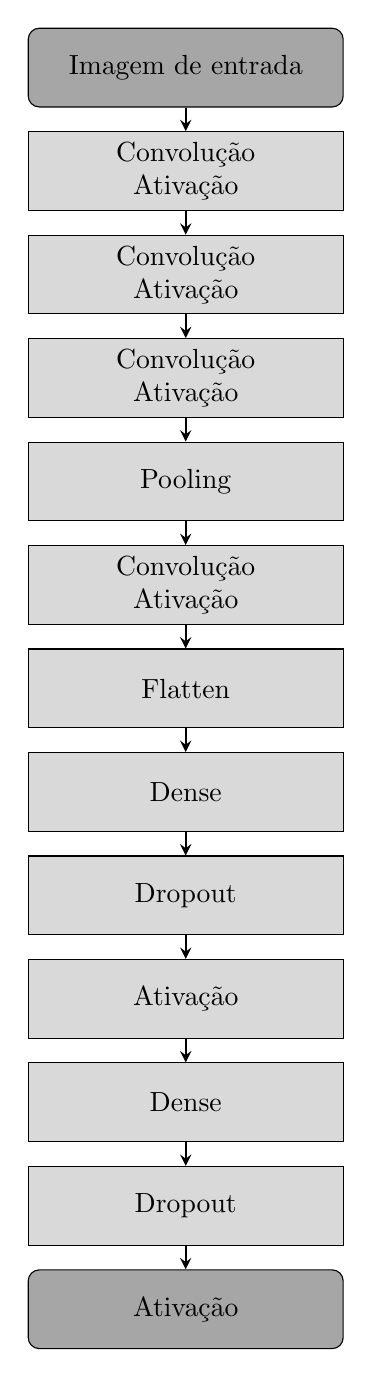
\begin{tikzpicture}[
	start chain=going below,
	every join/.style={arrow},
	node distance=0.3cm
	]
	\node (start) [startstop,on chain,join] {Imagem de entrada};
	
	\node (out1) [process,on chain,join] {Convolução \\ Ativação};
	
	\node (out3) [process,on chain,join] {Convolução \\ Ativação };
	
	\node (out5) [process,on chain,join] {Convolução \\ Ativação};
	
	\node (out7) [process,on chain,join] {Pooling};
	
	\node (out8) [process,on chain,join] {Convolução \\ Ativação};
	
	\node (out10) [process,on chain,join] {Flatten};
	\node (out11) [process,on chain,join] {Dense};
	
	\node (out12) [process,on chain,join] {Dropout};
	\node (out13) [process,on chain,join] {Ativação};	
	
	\node (out14) [process,on chain,join] {Dense};
	\node (out15) [process,on chain,join] {Dropout};
	
	\node (out16) [startstop,on chain,join] {Ativação};		
	
	\end{tikzpicture}%
	} %resizebox
	\caption{Arquitetura da rede CNN utilizada neste trabalho.}
		\label{tikz:mnist_cnn16}
\end{figure}

\par A implementação da rede descrita pela imagem \ref{tikz:mnist_cnn16} é exibida no código abaixo:
\begin{lstlisting}
from keras.layers import Activation
from keras.layers.convolutional import Convolution2D, MaxPooling2D
from keras.layers import Flatten, Dense
from keras.layers.core import Dropout

dropout_rate=0.3

modelo = Sequential()

def keras_add(m,op):
	m.add(op)
	l = m.layers[-1]

keras_add(modelo,Convolution2D(32, 2, 2,
	border_mode='valid', input_shape=(28, 28, 1)))
keras_add(modelo,Activation('relu'))

keras_add(modelo,Convolution2D(8, 12, 12))
keras_add(modelo,Activation('relu'))

keras_add(modelo,Convolution2D(16, 8, 8))
keras_add(modelo,Activation('relu'))

keras_add(modelo,MaxPooling2D(pool_size=(2, 2)))

keras_add(modelo,Convolution2D(32, 2, 2))
keras_add(modelo,Activation('relu'))

keras_add(modelo,Flatten())
keras_add(modelo,Dense(100))
keras_add(modelo,Dropout(dropout_rate))
keras_add(modelo,Activation('relu'))

keras_add(modelo,Dense(numero_classes))
keras_add(modelo,Dropout(dropout_rate))
keras_add(modelo,Activation('softmax'))
\end{lstlisting}

\par O objetivo das camadas convolucionais com ativação no início dessa rede é de encontrar características dos números e reduzir parcialmente o tamanho da imagem inicial antes do primeiro \textit{pooling}. Para melhor compreensão dos efeitos da convolução nas imagens foram utilizados em cada camada convolucional filtros dos tamanhos: 32 filtros de 2x2, 8 filtros de 12x12, 16 filtros de 8x8 e 32 filtros de 2x2.

\par A visualização dos filtros obtidos após o treinamento foi obtida da seguinte forma:

\begin{lstlisting}
img = np.zeros((28,28))
for a in xrange(28):
  for b in xrange(28):
    img[a][b] = X_treino[0][a,b]
    for i in xrange(len(modelo.layers)):
      m0 = modelo.layers[i]
      name = m0.name
      if "convolution" not in name:
        continue    
      ws = m0.get_weights()

      flt = np.zeros((np.shape(ws[0])[0],np.shape(ws[0])[1]))
      fig=plt.figure(figsize=(8,8))
      for oz in xrange(np.shape(ws[0])[2]):
        for z in xrange(np.shape(ws[0])[3]):
          ax = fig.add_subplot(6, 6, z+1)
          sa = np.shape(ws[0])[0]
          sb = np.shape(ws[0])[1]
          for a in xrange(sa):
            for b in xrange(sb):
              flt[a][b] = ws[0][a,b,oz,z]
              plt.xticks(np.array([]))
              plt.yticks(np.array([]))
              plt.tight_layout()        
              ax.imshow(flt,interpolation='nearest', cmap=plt.cm.gray) 
\end{lstlisting}


\par Os filtros descritos acima são visualizados na imagem \autoref{fig:convs_filtros}.

\begin{figure}[H]
	\centering
	
	\begin{subfigure}{.8\textwidth}
		\centering
		\includegraphics[width=.6\linewidth]{images/fabio/resultados/network_3/filter_convolution2d_1}%
		\caption{Filtros 2x2 - primeira convolução}		
		\label{fig:conv1_filtro}	
	\end{subfigure}%
	
	\begin{subfigure}{.8\textwidth}
		\centering
		\includegraphics[width=.6\linewidth]{images/fabio/resultados/network_3/filter_convolution2d_2}
		\caption{Filtros 12x12 - segunda convolução}		
		\label{fig:conv2_filtro}	
	\end{subfigure}%
	
	\begin{subfigure}{.8\textwidth}
		\centering
		\includegraphics[width=.6\linewidth]{images/fabio/resultados/network_3/filter_convolution2d_3}%
		\caption{Filtros 8x8 - terceira convolução}		
		\label{fig:conv3_filtro}	
	\end{subfigure}%
d
	\begin{subfigure}{.8\textwidth}
	\centering
	\includegraphics[width=.6\linewidth]{images/fabio/resultados/network_3/filter_convolution2d_4}%
	\caption{Filtros 2x2 - terceira convolução}		
	\label{fig:conv4_filtro}	
\end{subfigure}%
	\caption{Filtros convolucionais obtidos do treinamento.}
		\label{fig:convs_filtros}
\end{figure}


\par Após as primeiras camadas de convolução foi adicionada uma camada de \textit{pooling} para auxiliar na eliminação de ruídos e reduzir o número de elementos a serem explorados pela rede.
\par A seguir, uma nova camada de convolução foi adicionada para detectar novas características novamente. Por conta da estrutura do \textit{framework} do Keras, utilizado neste trabalho é necessário antes da rede \textit{fully-connected} ou (\textit{dense}) transformar a entrada em um vetor unidimensional, representada mais a frente por uma fita.
\par A camada \textit{dense} trabalha como uma camada de redes neurais conectando todos os elementos da entrada com todos os elementos da saída, visando estabelecer a relação da importância entre os elementos ativados e os resultados obtidos.
\par O próximo elemento é uma camada de \textit{Dropout} com objetivo de minimizar a dependência de algumas características específicas dos dígitos. Em seguida é utilizada uma camada de ativação para evidenciar os elementos mais importantes encontrados após a camada \textit{dense+droupout}.
\par Os últimos dois passos são novamente uma camada \textit{dense}, agora reduzindo as entradas de 100 para 10 elementos  (correspondentes aos dígitos de 0 a 9) e uma nova camada de ativação agora com função \textit{softmax} para ativação de um único elemento (representando a escolha da rede do elemento mais provável identificado pela rede).

\par A identificação do dígito é iniciada com a introdução da imagem contendo o item a ser identificado. Neste exemplo será utilizado o número 0 apresentado na imagem \ref{fig:numero_0}.

\begin{center}
\begin{figure}[H]
	\centering
	\includegraphics[width=0.3\linewidth]{images/fabio/numero_0}
	\caption{Número 0 escrito a mão disponível na base de dados do MNIST.}
	\label{fig:numero_0}
\end{figure}
\end{center}


\par A aplicação do primeiro conjunto de camada convolucional e ativação é mostrada em \autoref{fig:camada_1}. Apesar da aplicação dos filtros não resultar necessariamente em uma imagem humanamente compreensível é possível notar na ativação da \ref{fig:camada_1} que as bordas ficam ressaltadas em relação ao fundo e algumas das camadas buscam encontrar formatos específicos como linhas horizontais e verticais enquanto outras buscam formatos de curvas. 

\begin{center}
\begin{figure}[H]
\centering
\begin{subfigure}{.8\textwidth}
\centering
\includegraphics[width=.6\linewidth]{images/fabio/resultados/network_3/filter_convolution2d_1}%
\caption{Filtros 2x2 aplicados a primeira camada de convolução}		
\label{fig:filtros2x2}	
\end{subfigure}%

\begin{subfigure}{.8\textwidth}
\centering
\includegraphics[width=.6\linewidth]{images/fabio/resultados/network_3/input_1_layer_convolution2d_1}
\caption{Convolução 1}
\end{subfigure}%

\begin{subfigure}{.8\textwidth}
\centering
\includegraphics[width=.6\linewidth]{images/fabio/resultados/network_3/input_1_layer_activation_1}%
\caption{Ativação}			
\end{subfigure}%
\caption{Primeiro resultado da identificação no primeiro par de camadas de convolução e ativação.}
\label{fig:camada_1}
\end{figure}
\end{center}

%%%%%%%%%%%%%%%%%%%%%%%%%%%%%%%%%%%%%%%%%%%%%%%%%%%

\par Na segunda camada um filtro de tamanho 12x12 é utilizado. Novamente, apesar de não necessariamente ser uma imagem compreensível para humanos é possível notar no próprio filtro que alguns formtados de curvas e traços ficam evidenciado, indicando que esses filtros irão se ativar mais para esse tipo de padrão. O resultado na \autoref{fig:camada_2} tem a resolução menor por conta da redução no tamanho da saída. A saída dessa segunda camada é composta por varios componentes do número zero como bordas internas e externas além da evidenciação do centro do zero.

\begin{center}
\begin{figure}[H]
\begin{subfigure}{.8\textwidth}
	\centering
	\includegraphics[width=.6\linewidth]{images/fabio/resultados/network_3/filter_convolution2d_2}%
	\caption{Filtros 12x12 aplicados a segunda camada de convolução}		
	\label{fig:filtros12x12}	
\end{subfigure}%

\begin{subfigure}{.8\textwidth}
	\centering
	\includegraphics[width=.6\linewidth]{images/fabio/resultados/network_3/input_1_layer_convolution2d_2}
	\caption{Convolução 2}
\end{subfigure}%

\begin{subfigure}{.8\textwidth}
	\centering
	\includegraphics[width=.6\linewidth]{images/fabio/resultados/network_3/input_1_layer_activation_2}%
	\caption{Ativação}			
\end{subfigure}%
\caption{Primeiro resultado da identificação no segundo par de camadas de convolução e ativação.}
\label{fig:camada_2}
\end{figure}
\end{center}
%%%%%%%%%%%%%%%%%%%%%%%%%%%%%%%%%%%%%%%%%%%%%%%%%%%

\par A terceira camada utiliza um filtro 8x8, dessa vez praticamente nenhum elemento dos filtros é humanamente compreensível. A convolução nesta camada mostra que aguns filtros buscam por um padrão onde as bordas são preenchidas e o entro é vazio, e alguns outros filtros que também são mais ativados evidenciam o formato circular que o número zero tem.
\begin{center}
\begin{figure}[H]
	\begin{subfigure}{.8\textwidth}
		\centering
		\includegraphics[width=.6\linewidth]{images/fabio/resultados/network_3/filter_convolution2d_3}%
		\caption{Filtros 8x8 aplicados a terceira camada de convolução}		
		\label{fig:filtros8x8}	
	\end{subfigure}%
	
	\begin{subfigure}{.8\textwidth}
		\centering
		\includegraphics[width=.6\linewidth]{images/fabio/resultados/network_3/input_1_layer_convolution2d_3}
		\caption{Convolução 3}
	\end{subfigure}%
	
	\begin{subfigure}{.8\textwidth}
		\centering
		\includegraphics[width=.6\linewidth]{images/fabio/resultados/network_3/input_1_layer_activation_3}%
		\caption{Ativação}			
	\end{subfigure}%
	\caption{Primeiro resultado da identificação no terceiro par de camadas de convolução e ativação.}
		\label{fig:camada_3}
\end{figure}
\end{center}
%%%%%%%%%%%%%%%%%%%%%%%%%%%%%
\par A camada de \textit{pooling} tem como objetivo reduzir a dimensionalidade como é visto na \autoref{fig:input1layermaxpooling2d1}. O resultado da imagem com alguns dos filtro não possuem nenhum valor (filtro 5/16)=, enquanto outros capturam mais os pares de bordas (filtros 1/16 e 2/16) e outros apenas algumas bordas (filtros 14/16 e 15/16).

\begin{center}
\begin{figure}[H]
	\centering
	\includegraphics[width=0.5\textwidth]{images/fabio/resultados/network_3/input_1_layer_maxpooling2d_1}
	\caption{Resultado da camada de Pooling}
	\label{fig:input1layermaxpooling2d1}
\end{figure}
\end{center}

%%%%%%%%%%%%%%%%%%%%%%%%%%%%%%%%%%%%%%%%%%%%%%%%%%%
\par Na quarta camada de convolução o resultado é uma imagem de 3x3 pixels. Não é possível afirmar exatamente o que cada resultado representa (por conta da forma como o aprendizado de máquina funciona), mas é possível verificar que o ponto mais ativo em cada filtro  representa uma relação dentre cada um dos 9 pixels da imagem e os elementos adjacentes.

\begin{center}
\begin{figure}[H]
	\begin{subfigure}{.8\textwidth}
		\centering
		\includegraphics[width=.6\linewidth]{images/fabio/resultados/network_3/filter_convolution2d_4}%
		\caption{Filtros 2x2 aplicados a quarta camada de convolução}		
		\label{fig:filtros2x2_4}	
	\end{subfigure}%
	
	\begin{subfigure}{.8\textwidth}
		\centering
		\includegraphics[width=.6\linewidth]{images/fabio/resultados/network_3/input_1_layer_convolution2d_4}
		\caption{Convolução 4}
	\end{subfigure}%
	
	\begin{subfigure}{.8\textwidth}
		\centering
		\includegraphics[width=.6\linewidth]{images/fabio/resultados/network_3/input_1_layer_activation_4}%
		\caption{Ativação}			
	\end{subfigure}%
	\caption{Primeiro resultado da identificação no quarto par de camadas de convolução e ativação.}
		\label{fig:camada_2}
\end{figure}
\end{center}
%%%%%%%%%%%%%%%%%%%%%%%%%%%%%%%%%%%%%
\par A função Flatten do Keras, \autoref{fig:input1flatten}, transformar um item multidimensional em um vetor unidimensional. Neste caso 3x3x32 (imagem 3x3 e 32 filtros) transformasse em um vetor 1x1x288. Este artifício é utilizado para pode realizar a interface com a camada de treinamento \textit{fully connected} (totalmente conectada) assim como no aprendizado clássico de redes neurais.
\begin{center}
\begin{figure}[H]
	\centering
	\includegraphics[width=0.5\textwidth]{images/fabio/resultados/network_3/input_1_layer_flatten_1}
	\caption{Resultado da camada de Flatten}
	\label{fig:input1flatten}
\end{figure}
\end{center}

%%%%%%%%%%%%%%%%%%%%%%%%%%%%%%%%%%%%%
\par A camada Dense do Keras, \autoref{fig:input1dense1}, representa o treinamento clássico de redes neurais onde cada elemento da entrada é ligado a todos os elementos da camada escondida que por sua vez é ligado por todos os elementos de saída. Como as camadas anteriores reduziram a dimensionalidade da imagem o treinamento nesta fase é relativamente rápido por contar com 288 elementos de entrada e 100 elementos de saída apenas.
\begin{center}
\begin{figure}[H]
	\centering
	\includegraphics[width=0.5\textwidth]{images/fabio/resultados/network_3/input_1_layer_dense_1}
	\caption{Resultado da camada Dense}
	\label{fig:input1dense1}
\end{figure}
\end{center}


%%%%%%%%%%%%%%%%%%%%%%%%%%%%%%%%%%%%%
\par Uma camada de ativação é adicionada em \autoref{fig:input1atv5} com objetivo de passar para a próxima camada apenas os elementos mais importantes e eliminar possíveis ruídos no treinamento.
\begin{center}
\begin{figure}[H]
	\centering
	\includegraphics[width=0.5\textwidth]{images/fabio/resultados/network_1/input_1_layer_activation_7}
	\caption{Resultado da camada de ativação antes da saída}
	\label{fig:input1atv5}
\end{figure}
\end{center}
%%%%%%%%%%%%%%%%%%%%%%%%%%%%%%%%%%%%%
\par Uma nova camada Dense é adiciona agora para realizar a classificação entre 10 itens (número de 0 a 9).
\begin{center}
\begin{figure}[H]
	\centering
	\includegraphics[width=0.5\textwidth]{images/fabio/resultados/network_1/input_1_layer_dense_2}
	\caption{Resultado da camada de ativação antes da saída}
	\label{fig:input1dense2}
\end{figure}
\end{center}
%%%%%%%%%%%%%%%%%%%%%%%%%%%%%%%%%%%%%
\par A ultima camada de ativação elimina os outros resultados menos prováveis e mantém apenas o elemento que foi mais ativado. Neste caso apenas o único elemento do vetor com indice zero representando o número 0.
\begin{center}
\begin{figure}[H]
	\centering
	\includegraphics[width=0.5\textwidth]{images/fabio/resultados/network_1/input_1_layer_activation_8}
	\caption{Resultado da camada de ativação para definição da saída}
	\label{fig:input1atv7}
\end{figure}
\end{center}
% ---
% Conclusão
% ---
\chapter{Conclusão}
% ---

\par O resultado da arquitetura apresentada na seção anterior foi de 98.89\% para os elementos de treino da base do MNIST e de 99.06\% para os elementos de teste da mesma base. Tais resultados demonstram que a aplicação da técnica de redes convolucionais para este problema foi efetiva se comparando a outros bons resultados demonstrados em outras redes convolucionais em \citeonline{mnistlecunn}.



% ----------------------------------------------------------
% ELEMENTOS PÓS-TEXTUAIS
% ----------------------------------------------------------
%\postextual

% ----------------------------------------------------------
% Referências bibliográficas
% ----------------------------------------------------------
\bibliography{bibliografia}

% ----------------------------------------------------------
% Glossário
% ----------------------------------------------------------
%
% Consulte o manual da classe abntex2 para orientações sobre o glossário.
%
%\glossary

% ----------------------------------------------------------
% Apêndices
% ----------------------------------------------------------

% ---
% Inicia os apêndices
% ---
%\begin{apendicesenv}

% Imprime uma página indicando o início dos apêndices
%\partapendices

% ----------------------------------------------------------
%\chapter{Quisque libero justo}
% ----------------------------------------------------------

%\lipsum[50]

% ----------------------------------------------------------
%\chapter{Nullam elementum urna vel imperdiet sodales elit ipsum pharetra ligula
%ac pretium ante justo a nulla curabitur tristique arcu eu metus}
%% ----------------------------------------------------------
%\lipsum[55-57]
%
%\end{apendicesenv}
%% ---
%
%
%% ----------------------------------------------------------
%% Anexos
%% ----------------------------------------------------------
%
%% ---
%% Inicia os anexos
%% ---
%\begin{anexosenv}
%
%% Imprime uma página indicando o início dos anexos
%\partanexos
%
%% ---
%\chapter{Morbi ultrices rutrum lorem.}
%% ---
%\lipsum[30]
%
%% ---
%\chapter{Cras non urna sed feugiat cum sociis natoque penatibus et magnis dis
%parturient montes nascetur ridiculus mus}
%% ---
%
%\lipsum[31]
%
%% ---
%\chapter{Fusce facilisis lacinia dui}
%% ---
%
%\lipsum[32]
%
%\end{anexosenv}
%
%%---------------------------------------------------------------------
%% INDICE REMISSIVO
%%---------------------------------------------------------------------
%
%\phantompart
%
%\printindex
%
%%---------------------------------------------------------------------
%% Formulário de Identificação (opcional)
%%---------------------------------------------------------------------
%\chapter*[Formulário de Identificação]{Formulário de Identificação}
%\addcontentsline{toc}{chapter}{Exemplo de Formulário de Identificação}
%\label{formulado-identificacao}
%
%Exemplo de Formulário de Identificação, compatível com o Anexo A (informativo)
%da ABNT NBR 10719:2015. Este formulário não é um anexo. Conforme definido na
%norma, ele é o último elemento pós-textual e opcional do relatório.
%
%\bigskip
%
%\begin{tabular}{|p{9cm}|p{5cm}|}
%\hline
%\multicolumn{2}{|c|}{\textbf{\large Dados do Relatório Técnico e/ou científico}}\\
%\hline
%\multirow{4}{10cm}[24pt]{Título e subtítulo}& Classificação de segurança\\
%                   & \\
%                   \cline{2-2}
%                   & No.\\
%                   & \\
%				
%\hline
%Tipo de relatório & Data\\
%\hline
%Título do projeto/programa/plano & No.\\
%\hline
%\multicolumn{2}{|l|}{Autor(es)} \\
%\hline
%\multicolumn{2}{|l|}{Instituição executora e endereço completo} \\
%\hline
%\multicolumn{2}{|l|}{Instituição patrocinadora e endereço completo} \\
%\hline
%\multicolumn{2}{|l|}{Resumo}\\[3cm]
%\hline
%\multicolumn{2}{|l|}{Palavras-chave/descritores}\\
%\hline
%\multicolumn{2}{|l|}{
%Edição \hfill No. de páginas \hfill No. do volume \hfill Nº de classificação \phantom{XXXX}} \\
%\hline
%\multicolumn{2}{|l|}{
%ISSN \hfill \hfill Tiragem \hfill Preço \phantom{XXXXXXXX}} \\
%\hline
%\multicolumn{2}{|l|}{Distribuidor} \\
%\hline
%\multicolumn{2}{|l|}{Observações/notas}\\[3cm]
%\hline
%\end{tabular}

\end{document}
